\begin{savequote}[80mm]
---Allora dovresti dire quello a cui credi---, riprese la Lepre Marzolina. \\
---È quello che faccio---, rispose subito Alice; \\
---almeno credo a quello che dico, che poi è la stessa cosa.--- \\
---Non è affatto la stessa cosa!--- disse il Cappellaio. \\
---Scusa, è come se tu dicessi che vedo quello che mangio è la stessa cosa di mangio quello che vedo!---
\qauthor{Lewis Carroll} \end{savequote}


\chapter{Logica Multimodale Classica	}


\section{Critiche al vecchio regime}

Nella logica modale, come l'abbiamo descritta nei precedenti capitoli,
sono possibili interpretazioni talvolta sgradite quando si danno significati
particolari agli operatori modali.
\begin{itemize}
\item $\boxx{\top}$ (schema N)
\end{itemize}
Sembra inappuntabile se $\square$ si legge come ``è possibile'' 

Ma diventa già discutibile se $\square$ si legge come ``è dimostrabile'',
infatti il teorema di goedel asserisce che non tutto ciò che è vero
è dimostrabile
\begin{itemize}
\item $\boxx{(a\wedge b)\implies\boa\wedge\boxx b}$ (schema \textbf{M})
\end{itemize}
Se diamo a $\square$ il significato di ``non so'' notiamo che questa
formula non è necessariamente significativa 

es. io non so se tizio sia allegro E un astronauta però so che è allegro
e quindi il conseguente in questo caso non è vero.
\begin{itemize}
\item $\boa\wedge\boxx b\implies\boxx{(a\wedge b)}$ (schema \textbf{C})
\end{itemize}
Analogo al precedente con ``vedo'' come $\square$


\section{Yet another Model}

A questo proposito si definisce diversamente il concetto di frame:

$F=(S,N)$ 

$S$ sia un insieme di stati 

$N:S\rightarrow\mathcal{P}(\mathcal{P}(S))$

e in modo naturale il modello $M=(S,N.V)$ che fissa una funzione
di verità

Si definisce insieme di verità di $a$ il seguente: $\verins a=\{\alpha:\ \veraw M{\alpha}{a\}}$

Inoltre diciamo che:

$\veraw M{\alpha}{\boxx a}$ se e solo se: $\verins a\in N(\alpha)$	

$\veraw M{\alpha}{\dia}$ se e solo se: $(S-\verins a)\notin N(\alpha)$	


\subsection{Negazione di N}

Ts) $\nonvera F{\boxx T}$\\


Consideriamo un frame con due stati$F(\{\alpha,\beta\},N)$

$N(\alpha)=\{\{\beta\}\}$

$N(\beta)=\{\{\alpha\},\{\beta\},\{\alpha,\beta\}\}$ (solo un esempio,
qualunque $N(\beta)$ va bene per la dimostrazione)

$\verins T=\{\alpha,\beta\}$ infatti $T$ è vero in ogni mondo, ma
$\nonveraw M{\alpha}{\boxx T}$ 

infatti $\verins T\notin N(\alpha)$


\subsection{Validità di N}

$\vera F{\boxx{\top}}$ se e solo se $S\in N(\alpha)\,\forall\alpha\in S$

Un frame in cui vale l'assioma N si dice frame con unità.


\subsection{Negazione di M}

Ts) $\nonvera F{\boxx{(a\wedge b)\implies\boa\wedge\boxx b}}$\\


Considero un frame in cui vale l'antecedente:

$S=\{\alpha,\beta\}$

$N(\alpha)=\emptyset$

$N(\beta)=\{\{\alpha,\beta\}\}$

$V(A)=\alpha$, $V(B)=\beta$

Con queste ipotesi si ha: $\veraw M{\alpha}{\boxx{(A\wedge B)}}$

infatti $\verins{A\wedge B}=\{\gamma:\ \mbox{\ensuremath{\veraw M{\gamma}{A\wedge B}}\}}$
= $\emptyset$ perché in nessuno mondo è vera sia A che B

e quindi:	$\verins{A\wedge B}\in N(\alpha)$ 

Ora mostro che non vale il conseguente:

$\verins A=\{\alpha\}$ e palesemente $\{\alpha\}\notin N(\alpha)=\emptyset$
da cui $\nonveraw M{\alpha}{\boxx A}$ da qui quindi neppure:

$\nonveraw M{\alpha}{\boxx{A\wedge\boxx B}}$


\subsection{Validità di M}

Ip)$\vera F{\boxx{(a\wedge b)\implies\boa\wedge\boxx b}}$ 

Ts)$\forall X,Y\ Se\ X\cap Y\in N(\alpha)\ allora\ X\in N(\alpha),\ Y\in N(\beta)$	\\
		

Considero un frame generico F che abbia $\alpha$ come stato

Siano $X,Y$ due insiemi di stati tali che

$X\cap Y\in N(\alpha)$. 

$V(A)=\{s\ |\ s\in X\}$

$V(B)=\{s\ |\ s\in Y\}$

Dato che $X\cap Y\in N(\alpha)$

si ha che$\verins{A\wedge B}\in N(\alpha)$, infatti $\verins{A\wedge B}=\{\gamma\ :\ \veraw M{\gamma}{A\wedge B\}}=\{s\ :\ s\in X\ e\ s\in Y\}=\{s\ :\ s\in X\cap Y\}=X\cap Y$

cioè gli stati in cui è vera $A\wedge B$ sono gli stati in cui vale
sia $A$ che $B$ cioè quelli che appartengono sia a $X$ che a $Y$

Si ha quindi $\veraw M{\alpha}{\boxx{(A\wedge B)}}$ da cui per ipotesi:

$\veraw M{\alpha}{\boa\wedge\boxx b}$ e cioè: $\veraw M{\alpha}{\boa}$
e $\veraw M{\alpha}{\boxx b}$ da cui:

$\verins A=\{\alpha:\ \veraw M{\alpha}A\}=X\in N(\alpha)$

$\verins B=\{\alpha:\ \veraw M{\alpha}B\}=Y\in N(\alpha)$	\\
\\
Ip)$\forall X,Y\ Se\ X\cap Y\in N(\alpha)\ allora\ X\in N(\alpha),\ Y\in N(\beta)$

Ts)$\vera F{\boxx{(a\wedge b)\implies\boa\wedge\boxx b}}$\\


Supponiamo valga $\veraw M{\alpha}{\boxx{(a\wedge b)}}$ allora: \\
$\verins{a\wedge b}\in N(\alpha)$ (per definizione di $\square)$,
da cui:

$\verins a\cap\verins b\in N(\alpha)$, se chiamo $X$ e $Y$ questi
insiemi di verità allora ho per ipotesi

$\verins a\in N(\alpha)$ e $\verins b\in N(\alpha)$,

dalla prima, per definizione di $\square$ ottengo $\veraw M{\alpha}{\boa}$

dalla seconda ottengo $\veraw M{\alpha}{\boxx b}$ 

quindi complessivamente $\veraw M{\alpha}{\boa\wedge\boxx b}$\\


Un frame in cui valga l'assioma M si dice frame supplementato.


\subsection{Negazione di C}

Ts) $\vera FC$\\


Consideriamo un frame con due stati $F(\{\alpha,\beta\},N)$ e la
seguente valutazione:

$N(\alpha)=\{\{\beta\},\,\{\alpha\}\}$

$V(A)=\{\beta\}$

$V(B)=\{\alpha\}$

avremo dunque che:

$\veraw{\mu}{\alpha}{\boa}$

$\veraw{\mu}{\alpha}{\boxx b}$

ma non vale:

$\nonveraw{\mu}{\alpha}{\boxx{}(A\wedge B)}$

infatti:

$\emptyset\nsubseteq N(\alpha)$


\subsection{Validità di C}

Ip) $\vera FC$ 

Ts) $\forall\alpha\in S,\,\forall X,\, Y\subseteq S\,:\, X\cap Y\in N(\alpha)$\\


Poiché vale l'assioma C possiamo scrivere:

$\vera F{\boxx A\wedge\boxx B}\implies\boxx{(A\wedge B)}$

supponiamo valga l'antecedente, allora supponendo:

$V(A)=\{s\,|\, s\in X\}$

$V(B)=\{s\,|\, s\in Y\}$

Avremo che:

$\verins A=X$

$\verins B=Y$

Ma per modus ponens vale il conseguente, e quindi:

$\veraw{\mu}{\alpha}{\boxx{(A\wedge B)}}$

e quindi l'insieme di verità:

$\verins{A\wedge B}\in N(\alpha)$

da cui segue:

$(X\cap Y)\in N(\alpha)$

e la tesi è dimostrata.

Ip) $\forall\alpha\in S,\,\forall X,\, Y\subseteq S\,:\, X\cap Y\in N(\alpha)$

Ts) $\vera FC$ \\


Se l'antecedente è falso, C è vero, per cui consideriamo il caso in
cui valga la formula:

$\veraw{\mu}{\alpha}{\boa\wedge\boxx b}$

avremo quindi che:

$\verins A\in N(\alpha)$

$\verins B\in N(\alpha)$

allora possiamo scrivere:

$\verins A\cap\verins B\equiv\verins{A\wedge B}\in N(\alpha)$\\


Un frame in cui valga l'assioma C si dice chiuso rispetto all'intersezione.


\subsection{Proprietà dei frame}

Un frame si quasi filtro se:
\begin{enumerate}
\item È supplementato
\item Èchiuso rispetto all'intersezione
\end{enumerate}
Un frame si dice filtro se:
\begin{enumerate}
\item È un quasi filtro
\item È un frame con unità
\end{enumerate}

\section{Logiche Classiche}

Le logiche classiche sono tutte le logiche valide sui frame minimali.
La minima logica classica è la Logica E.

La logica è è definita come la logica che:
\begin{itemize}
\item Contiene tutte le tautologie
\item E' chiusa rispetto al Modus Ponens
\item E' chiusa rispetto alla regola RE
\end{itemize}
RE: $\dfrac{a\iff b}{\boa\iff\boxx b}$

Le logiche Monotone sono logiche classiche in cui vale anche la regola
RM:

RM: $\dfrac{a\implies b}{\boa\implies\boxx b}$

Le logiche Regolari sono logiche classiche in cui vale la regola RR:

RR: $\dfrac{a\wedge b\implies c}{\boa\wedge\boxx b\implies\boxx b}$


\subsection{Reticolo delle logiche classiche}

\begin{center} 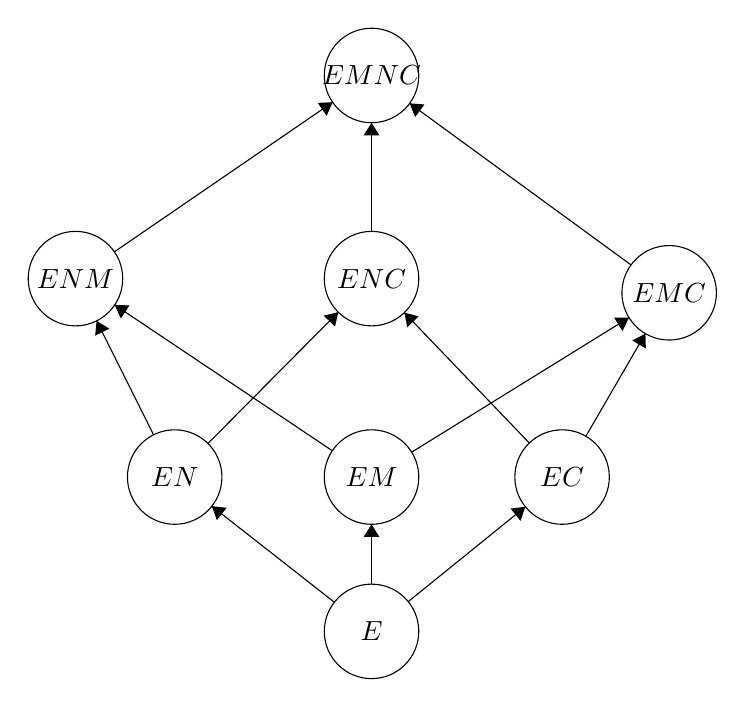
\begin{tikzpicture}[scale=0.2] \tikzstyle{every node}+=[inner sep=0pt] \draw [black] (37.1,-46.6) circle (3); \draw (37.1,-46.6) node {$E$}; \draw [black] (24.6,-36.8) circle (3); \draw (24.6,-36.8) node {$EN$}; \draw [black] (37.1,-36.8) circle (3); \draw (37.1,-36.8) node {$EM$}; \draw [black] (49.2,-36.8) circle (3); \draw (49.2,-36.8) node {$EC$}; \draw [black] (18.3,-24.2) circle (3); \draw (18.3,-24.2) node {$ENM$}; \draw [black] (37.1,-24.2) circle (3); \draw (37.1,-24.2) node {$ENC$}; \draw [black] (56,-25.1) circle (3); \draw (56,-25.1) node {$EMC$}; \draw [black] (37.1,-11.3) circle (3); \draw (37.1,-11.3) node {$EMNC$}; \draw [black] (37.1,-43.6) -- (37.1,-39.8); \fill [black] (37.1,-39.8) -- (36.6,-40.6) -- (37.6,-40.6); \draw [black] (34.74,-44.75) -- (26.96,-38.65); \fill [black] (26.96,-38.65) -- (27.28,-39.54) -- (27.9,-38.75); \draw [black] (39.43,-44.71) -- (46.87,-38.69); \fill [black] (46.87,-38.69) -- (45.93,-38.8) -- (46.56,-39.58); \draw [black] (34.61,-35.13) -- (20.79,-25.87); \fill [black] (20.79,-25.87) -- (21.18,-26.73) -- (21.73,-25.9); \draw [black] (23.26,-34.12) -- (19.64,-26.88); \fill [black] (19.64,-26.88) -- (19.55,-27.82) -- (20.45,-27.38); \draw [black] (39.65,-35.22) -- (53.45,-26.68); \fill [black] (53.45,-26.68) -- (52.51,-26.68) -- (53.03,-27.53); \draw [black] (50.71,-34.21) -- (54.49,-27.69); \fill [black] (54.49,-27.69) -- (53.66,-28.13) -- (54.52,-28.64); \draw [black] (26.71,-34.67) -- (34.99,-26.33); \fill [black] (34.99,-26.33) -- (34.07,-26.55) -- (34.78,-27.25); \draw [black] (47.12,-34.64) -- (39.18,-26.36); \fill [black] (39.18,-26.36) -- (39.37,-27.29) -- (40.09,-26.59); \draw [black] (20.77,-22.5) -- (34.63,-13); \fill [black] (34.63,-13) -- (33.68,-13.04) -- (34.25,-13.86); \draw [black] (37.1,-21.2) -- (37.1,-14.3); \fill [black] (37.1,-14.3) -- (36.6,-15.1) -- (37.6,-15.1); \draw [black] (53.58,-23.33) -- (39.52,-13.07); \fill [black] (39.52,-13.07) -- (39.87,-13.94) -- (40.46,-13.14); \end{tikzpicture} \end{center} 

EM è la minima logica monotona

EMC è la minima logica regolare

$EMNC\equiv K$ è la minima logica normale


\subsection*{Teorema}

Le logiche normali sono regolari, le logiche regolari sono monotone,
le logiche monotone sono classiche.

Ip) Vale K

Ts) la logica è regolare\\


$\teoremaDi Ka\wedge b\implies c$ -- per ipotesi

$\teoremaDi K\boxx{(a\wedge b)}\implies\boxx c$ --definizione 3.c
di logica normale

$\teoremaDi K\boa\wedge\boxx b\implies\boxx{(a\wedge b)}$ -- perché
è una logica nomale (definizione 3.b)

$\teoremaDi K\boa\wedge\boxx b\implies\boxx c$ -- per catena di implicazioni
fra le due precedenti

Poiché vale RR, ogni logica normale è regolare

Ip) Vale la regola RR

Ts) Vale la regola RM\\


$\teorema{a\implies b}$ -- per ipotesi

$\teorema{a\wedge a\implies b}$ -- tautologia

$\teorema{\boa\wedge\boa\implies\boxx b}$ -- per RR

$\teorema{\boa\implies\boxx b}$ 

Poiché vale RM, ogni logica regolare è monotona

Ip) Vale RM

Ts) Vale RE\\


$\teorema{a\iff b}$ -- per ipotesi

$\teorema{a\implies b}$

$\teorema{b\implies a}$

$\teorema{\boa\implies\boxx b}$ -- per RM

$\teorema{\boxx b\implies\boa}$ -- per RM

$\teorema{\boa\iff\boxx b}$

Poiché vale RE, ogni logica monotona è classica


\subsection{Minima logica monotona}

La minima logica monotona è EM, ossia la logica E con l'aggiunta dell'assioma
M

Ip) valgono RE e M

Ts) vale RM\\


$\teorema{a\implies b}$ -- per ipotesi

$\teorema{(a\implies b)\implies(a\iff(a\wedge b))}$ -- per tautologia

$\teorema{a\iff(a\wedge b)}$ -- per MP 

$\teorema{\boa\iff\boxx{(a\wedge b)}}$ -- per RE

$\teorema{\boxx{(a\wedge b)\implies\boa\wedge\boxx b}}$ -- schema
M

$\teorema{\boa\implies\boa\wedge\boxx b}$ -- per MP

$\teorema{\boa\implies\boxx b}$

E il teorema è dimostrato

Ip) vale RM

Ts) Vale M\\


$\teorema{a\wedge b\implies a}$ -- per tautologia

$\teorema{a\wedge b\implies b}$ -- per tautologia

$\teorema{\boxx{(a\wedge b)\implies\boa}}$ -- per RM

$\teorema{\boxx{(a\wedge b)}\implies\boxx b}$ -- per RM

$\teorema{\boxx{(a\wedge b)\implies\boa\wedge\boxx b}}$ 

Che è lo schema M, e la tesi è dimostrata


\subsection{Minima logica regolare}

La minima logica regolare è EMC, ossia la logica E con l'aggiunta
degli assiomi M e C

Ip) valgono RE, M e C

Ts) vale RR\\


Sappiamo già che da RE e M ottengo RM.

$\teorema{a\wedge b\implies c}$ -- per ipotesi

$\teorema{\boxx{(a\wedge b)}\implies\boxx c}$ -- per RM

$\teorema{\boa\wedge\boxx b\implies\boxx{(a\wedge b)}}$ -- schema
C

$\teorema{\boa\wedge\boxx b\implies\boxx c}$ -- per MP

Poiché vale RR, la tesi è dimostrata.

Ip) vale RR

Ts) valgono M e C\\


Poiché abbiamo RR, sappiamo che vale RM, ma allora sappiamo già che
vale RE e l'assioma M.

$\teorema{a\wedge b\implies a\wedge c}$ -- per tautologia

$\teorema{\boa\wedge\boxx b\implies\boxx{a\wedge c}}$ -- per RR

Abbiamo trovalo lo schema C, quindi la tesi è dimostrata.


\subsection{Minima logica normale}

La minima logica normale è EMCN, ossia la logica E con l'aggiunta
dei tre assiomi M, C e N.

Questa logica è equivalente alle logiche normali, ossia i tre assiomi
insieme sono equivalenti alla logica K.

Ip) valgono RE, M, C, N

Ts) vale la logica K\\


Possiamo notare che, per definizione della logica K, devono valere:
\begin{itemize}
\item N 
\item C
\item $(a\implies b)\implies(\boa\implies\boxx b)$
\end{itemize}
Resta soltanto l'ultima affermazione da dimostrare.

Sappiamo già che con RE e M otteniamo RM, e quindi:

$\teorema{a\implies b}$ -- per ipotesi

$\teorema{\boa\implies\boxx b}$ -- per RM

Ip) vale K

Ts) vale RE, M, C e N.\\


Poiché siamo in una logica normale vale RR e quindi valgono RE, M
e C.

N vale per punto 1 della definizione di logica normale.

La tesi è quindi dimostrata.


\section{Relazione Tra Frame Minimali E Standard}

Poiché le logiche classiche contengono le logiche normali, è possibile
delineare la relazione tra i frame minimali e i frame standard.


\subsection{Frame Aumentato}

Si dice frame aumentato, un frame F supplementato tale che:

$\forall\alpha\, Z\equiv\underset{Y\in N(\alpha)}{\bigcap}Y\, Z\in N(\alpha)$	

Un frame aumentato è un filtro:
\begin{enumerate}
\item è supplementato
\item è chiuso rispetto all'intersezione
\item non è vuoto (c'è sempre almeno il vuoto)
\end{enumerate}

\subsection{Teorema}

Per ogni modello minimale aumentato $\mu^{a}=(S,\, N,\, V)$ esiste
un modello standard $\mu^{s}=(S,\, R,\, V)$ tale che, $\forall\alpha\in S$
e $\forall a\in f.b.f$

$\veraw{\mu^{a}}{\alpha}a\iff\veraw{\mu^{s}}{\alpha}a$

Questo teorema è banalmente vero per le formule che non utilizzano
i connettivi modali, poiché S e V sono identiche. Dobbiamo dimostrarlo
solo nel caso di utilizzo dei connettivi modali, e poi per induzione
sulla complessità della formula, si può verificare che il teorema
è valido in generale.

Ip) $\veraw{\mu^{a}}{\alpha}a$

Ts) $\exists\mu^{s}\,:\,\veraw{\mu^{s}}{\alpha}a\iff\veraw{\mu^{a}}{\alpha}a$\\


Supponiamo di scegliere R tale che:

$(\alpha,\,\beta)\in R\iff\beta\in\underset{Y\in N(\alpha)}{\bigcap}Y$

abbiamo che:

$\veraw{\mu^{a}}{\alpha}{\boxx b\iff\verins b\in N(\alpha)}$

ma:

$\verins b\supseteq\underset{Y\in N(\alpha)}{\bigcap}Y$

allora possiamo affermare che:

$\forall\beta\,:\,(\alpha,\,\beta)\in R,\,\veraw{\mu^{s}}{\beta}b$

e quindi vale:

$\veraw{\mu^{s}}{\alpha}{\boxx{\beta}}$

viceversa, se è vero:

$\veraw{\mu^{s}}{\alpha}{\boxx b}$

allora avremo che:

$\veraw{\mu^{s}}{\beta}b$, $\forall\beta\,:\,(\alpha,\,\beta)\in R$

ma per definizione:

$\{\beta\,|\,(\alpha,\,\beta)\in R\}=\underset{Y\in N(\alpha)}{\bigcap}Y$

e allora:

$\verinsx bs=\verinsx ba\supseteq\underset{Y\in N(\alpha)}{\bigcap}Y$

e dunque:

$\veraw{\mu^{a}}{\alpha}a$

Ip) $\veraw{\mu^{s}}{\alpha}a$

Ts) $\exists\mu^{a}\,:\,\veraw{\mu^{a}}{\alpha}a\iff\veraw{\mu^{s}}{\alpha}a$\\


Supponiamo di scegliere N tale che:

$X\in N(\alpha)\iff X\supseteq\{\beta\,|\,(\alpha,\,\beta)\in R\}$

supponiamo che valga:

$\veraw{\mu^{s}}{\alpha}{\boxx b}$

e quindi:

$\veraw{\mu^{s}}{\beta}b$

ma allora abbiamo che:

$\verinsx bs\supseteq\{\beta\,|\,(\alpha,\,\beta)\in R\}$

ma allora abbiamo, per come abbiamo definito N:

$\verinsx ba\in N(\alpha)$

e quindi:

$\veraw{\mu^{a}}{\alpha}{\boxx b}$

viceversa, supponiamo di avere:

$\veraw{\mu^{a}}{\alpha}{\boxx b}$

allora per definizione avremo che:

$\verinsx ba\in N(\alpha)$

ma per come abbiamo definito N, si ha che:

$\verinsx ba\supseteq\{\beta\,|\,(\alpha,\,\beta)\in R\}$

ma allora abbiamo che:

$\verinsx ba=\verinsx bs$

da cui si ricavano banalmente:

$\veraw{\mu^{s}}{\beta}b$

$\veraw{\mu^{s}}{\alpha}{\boxx b}$

e la tesi è dimostrata.
